%---------------- distribution_0_1_metrique_wil_shapelets_P_len4950 ------------------
\begin{figure}[htb!] 
\centering
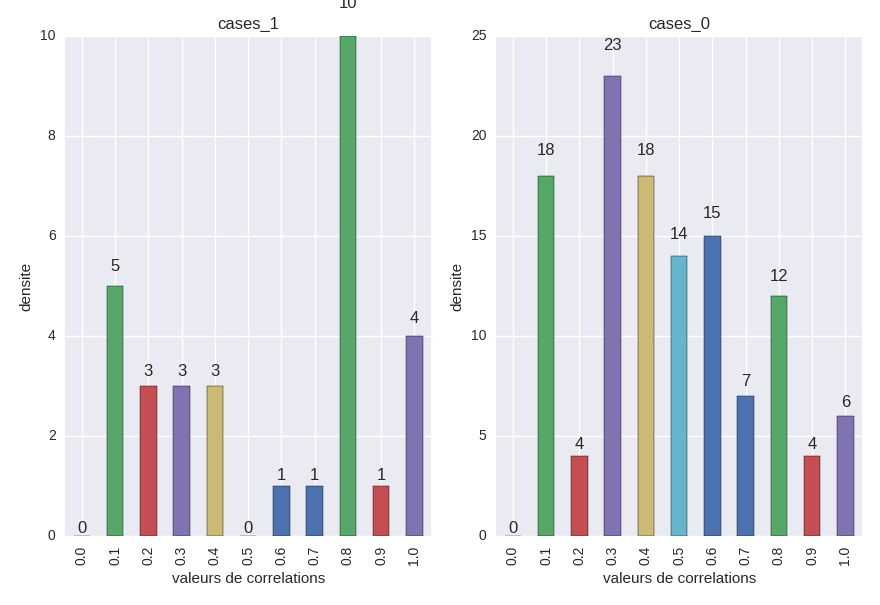
\includegraphics[width=500pt,height=250pt]{distribution_0_1_metrique_wil_shapelets_P_len4950.jpeg}
\caption{ Distribution des valeurs de corr\'elation de $M_c$ selon les cases \`a $0$ (\`a gauche) et \`a $1$ (\`a droite) de $M_{LG}$. La corr\'elation \`a $0.1$ d\'esigne  les valeurs de corr\'elation comprises entre $0.10$ et $0.199$. }
\label{distribution_0_1_metrique_wil_shapelets_P_len4950} 
\end{figure}
% \FloatBarrier
%---------------- distribution_0_1_metrique_wil_shapelets_P_len4950 ------------------


Soient la matrice $M_{LG}$ d'adjacence du line-graphe $LG$ du DAG non orient\'e de {\em Champlan} et $M_c$ sa matrice de corr\'elation obtenue avec la {\em distance de Pearson}.
 La distribution de valeurs de $M_c$ est repr\'esent\'ee par la figure \ref{distribution_0_1_metrique_wil_shapelets_P_len4950}. Le graphique \`a gauche de la figure \ref{distribution_0_1_metrique_wil_shapelets_P_len4950}  est la distribution des valeurs de $M_c$ selon les cases \`a $1$ dans $M_{LG}$ et le graphique \`a droite est celui des cases \`a $0$ dans $M_{LG}$. 
 Par exemple, la valeur de corr\'elation $0.1$ d\'esigne toutes les valeurs appartenant \`a $[0.1, 0.2[$. 
% En d'autres termes, ces distributions sont les celles des valeurs des cases {\em vrai n\'egatives} et {\em vrai positives}.
\newline
La densit\'e des  corr\'elations est d\'ecroissante pour les cases \`a $0$ quand les valeurs de corr\'elation tendent vers $1$. De m\^eme, cette densit\'e est croissante pour les cases \`a $1$ quand les corrections tendent vers $1$. La matrice $M_c$ contient des cases \'erron\'ees et ces cases ont une influence sur le calcul des valeurs de corr\'elation. C'est pourquoi les distributions ne sont pas lin\'eairement croissantes ou d\'ecroissantes.
Nous d\'ecidons, avec nos constatations, que la g\'en\'eration des distributions des valeurs de corr\'elation des cases \`a $0$ et $1$ suivent des lois normales asym\'etriques.
\newline

Nous  g\'en\'erons des valeurs de corr\'elation qui sont similaires \`a la distribution conjectur\'ee des valeurs de corr\'elation  du graphe de {\em Champlan}. Nous supposons que les valeurs de corr\'elation des cases \`a $0$ de $M_{LG}$ suivent la loi asym\'etrique de param\`etre $\alpha = 5$ et les valeurs de corr\'elation  des cases \`a $1$ de $M_{LG}$ suivent  cette m\^eme loi avec $\alpha = -5$ comme illustr\'e dans la figure \ref{distributionsCases01avecCoefficientAsymetries}. 
%---------------- distributionsCases01avecCoefficientAsymetries ------------------
\begin{figure}[htb!] 
\centering
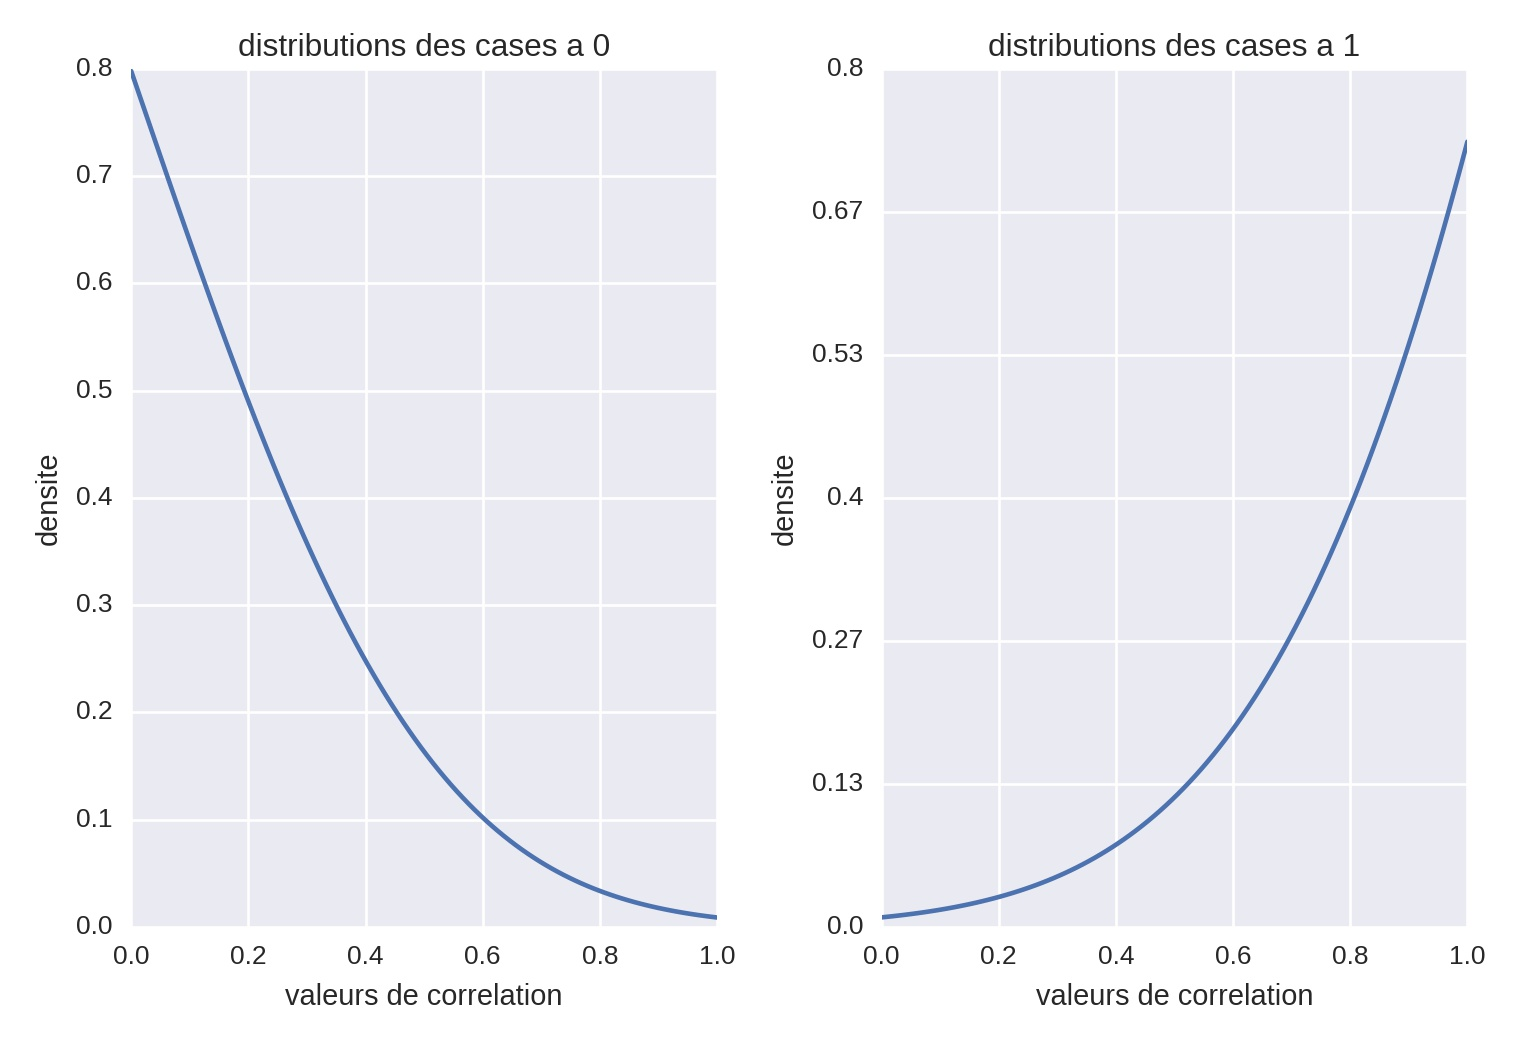
\includegraphics[width=500pt,height=250pt]{distributionsCases01avecCoefficientAsymetries.jpeg}
\caption{ Distribution des cases \`a $0$ et \`a $1$. \`A gauche : loi asym\'etrique de coefficient d'asym\'etrie $\alpha = 5$ pour les cases \`a $0$.  \`A droite : loi asym\'etrique de coefficient d'asym\'etrie $\alpha = -5$ pour les cases \`a $1$.}
\label{distributionsCases01avecCoefficientAsymetries} 
\end{figure}
% \FloatBarrier
%---------------- distributionsCases01avecCoefficientAsymetries ------------------
\newline

Soient 
$n_0$ la cardinalit\'e de l'ensemble des cases \`a $0$  de $M_{LG}$ et $n_1$ la cardinalit\'e de l'ensemble des cases \`a $1$ de $M_{LG}$.
Pour obtenir des valeurs de corr\'elation de $M_c$, nous g\'en\'erons  des valeurs r\'eelles $val$ appartenant \`a $[0,1]$ selon la loi asym\'etrique de coefficient $\alpha = 5$. Nous divisons l'intervalle $ [0,1]$ en $10$ sous-intervalles. Chaque sous-intervalle est not\'e  $]x_i,x_{i+1}]$ avec $x_i$ une valeur de corr\'elation et $i \in [0, 9]$. Nous calculons la densit\'e de chaque sous-intervalle et l'ensemble des densit\'es forme un histogramme qui suit une loi asym\'etrique.
Nous calculons la fonction de repartition $P$ de chaque densit\'e de telle sorte que 
$$
\forall x_i, x_{i+1}, P(X \le x_i) \le P(X \le x_{i+1}) ~~ et ~~ P(X \le x_{10}) = 1.
$$
\newline
Pour chaque case \`a $0$, nous tirons al\'eatoirement $n_0$ nombres r\'eels compris entre $0$ et $1$ uniformement. Si un nombre appartient \`a $]P(X \le x_i), P(X \le x_{i+1}) ]$ alors sa valeur de corr\'elation est $x_{i+1}$. Nous r\'ep\'etons les m\^emes \'etapes pour les cases \`a $1$ en g\'en\'erant les valeurs $val$ avec une loi asym\'etrique de coefficient $\alpha = -5$.
Nous obtenons la matrice de corr\'elation $M_c$ du line-graphe $LG$. Une distribution des valeurs de corr\'elation est repr\'esent\'ee par la figure \ref{distribution01} dans laquelle nous avons $189$ cases \`a $0$ et $111$ cases \`a $1$ dans $LG$.
%---------------- distribution01 ------------------
\begin{figure}[htb!] 
\centering
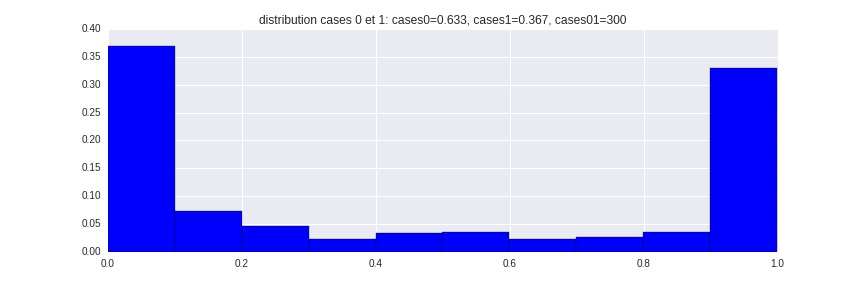
\includegraphics[width=550pt,height=250pt]{distribution01.jpeg}
\caption{ Un exemple de la distribution des valeurs de corr\'elations g\'en\'er\'ees. $63\%$ des cases sont des cases \`a 0 et $37\%$ sont des cases \`a $1$ dans $LG$.}
\label{distribution01} 
\end{figure}
% \FloatBarrier
%---------------- distribution01 ------------------

